%\emph{\emph{•}}
\documentclass{llncs}
%
\usepackage{amsmath}
\usepackage{amsfonts}
\usepackage{amssymb}
\usepackage{graphicx}
\usepackage{subcaption}
\captionsetup{compatibility=false}
\usepackage{url}
\usepackage[usenames]{color}

\newcommand{\keyterms}[1]{\par{\bfseries{ Key Terms: }}#1}

\begin{document}
\title{Distributed Datastores: Consistency Metric for Distributed Datastores}
\author{Kyrylo Rukkas\and Galyna Zholtkevych}
\institute{V.N.~Karazin Kharkiv National University\\
	4, Svobody Sqr., 61022, Kharkiv, Ukraine\\
	\email{galynazholtkevych1991@gmail.com}}
\maketitle
\begin{abstract}
Distributed databases being evolved require write requests to be handled independently to increase availability.
This means that nodes in a database can process modifying operation. This involves huge conflicts and leads to
full inconsistency and mess between replicas. This paper investigates a trade-off between availability and consistency
in a distributed database.
\end{abstract}

\section{Introduction}\label{sec:intro}
In the epoch of popular usage of IoT, Big Data, Cloud Computing, the data become more and more important thing and require larger, more reliable storage. This leads to increasing size of distributed storages. They become bigger and bigger and require the huge network across all the distributed nodes.
But there are several unsolved problems using large distributed datastores and some of them are strongly related to the CAP-theorem. 
Given that the ACID strategy can not be supported for systems of this class \cite{bib:brewer}, mechanisms for delivering data across distributed storage still lack fast eventual consistency convergence, reliability and tolerance to network partitions.

So let's concentrate on efficient consistency model - BASE (Basically Available, Soft State, Eventual Consistency) \cite{bib:acid_vs_base}
Mainly this paper is devoted to eventual consistency. Let us remind what eventual consistency is referencing to well-known book \cite{bib:tanenbaum}: the form of consistency is called eventual if no updates take place for a long time and all replicas will gradually become consistent.

Supporting replicas of an evolving distributed system up-to-date is very important but hard problem. Thus we need to provide a set of indicators of main characteristics of the distributed data store to assess the risk of a wrong decision because of the data inconsistency or unavailability.
In this paper, we focus our study on the problem of estimating data consistency in a distributed data store. Usually, in the datastore consistency is defined as binary for now. We want to demonstrate the useful concept defining of the consistency as binary value. 
For that instead of binary metric for eventual consistency/inconsistency we propose stochastic metric.

Also we would like to know if it is possible to find the optimal interval between writable operations occuring on distributed systems so that system can eventually be consistent in that interval.
In the section \ref{sec:model} we develop consistency model defined in the previous paper \cite{bib:prob_approach} and define the inconsistency metric for a distributed datastore.
In section \ref{sec:experiments} we conduct experiments that prove the correctness of metric defined in previous section.
In section \ref{sec:simulation} we provide diagrams of the implemented application that we use for carrying out experiments.
In section \ref{sec:complexity} section we approximate the time that is needed for consistency convergence - state of the distributed system when all nodes have consistent replicas.

%Given that in a distributed data store consistency of replicas may only be eventually \cite[{\color{red} you need to refer to the corresponding papers}]{?}, we need the answering the following questions
%\begin{enumerate}
%\item
%How to resolve conflicts between replicas?
%This problem is raised and partially solved in \cite{bib:c_ts}, where algorithm with timestamps on replicas is proposed.
%But merging updated replicas, it takes the response time, so consistency convergence decreases.
%In the paper further sections we will investigate faster consistency convergence.
%\item
%Is it always possible to ensure the convergence to the consistency of data and by what means can this be achieved?
%This depends on many factors including network topology,
%network failures, links bandwidth, bottlenecks in network overall etc \cite[{\color{red} links are needed}]{?}.
%\item
%What methods can be used to effectively solve the broadcast storm problem?
%This is well-known problem and it has the solution in \cite[{\color{red} links are needed}]{?}.
%\item How do loops when broadcasting data be eliminated?
%This is what networking algorithms aimed to solve \cite[{\color{red} links are needed}]{?}.
%\end{enumerate}

\section{Evolving consistency metric mathematical model: Derived metrics}\label{sec:model}

In the previous paper \cite{bib:prob_approach} we considered the metrics for all three elements of CAP-theorem.
Now our paper is mainly devoted to consistency question and how fast it can converge.
From that paper we are taking the developed mathematical model and expand it with elements, needed for the current research.

We specify it as a tuple $(N, L, \partial,D, r)$, where \\
\begin{tabular*}{\textwidth}{cp{0.5cm}p{0.8\textwidth}}
$N$&& is a finite set of nodes of a distributed datastore; \\
$L$&& is a finite set of links of a distributed datastore; \\
$\partial:L\rightarrow 2^N$&& is a mapping that associates each link with two nodes that it binds;\\
$D$&& is a finite set of stored data units;\\
$r:D\rightarrow 2^N$&& is a mapping that associates each data unit $d$ with a subset of nodes 
that store its replica; \\


$N_d$&& is a finite set of nodes that are having given dataunit $d$; \\
$l(N_d)$&& is a number of nodes in datastore that are having given dataunit; \\
$n_c$&& is a number of nodes in a subset of $N_d$ where all nodes have the same replica.
\end{tabular*}

So we expanded the model now with two last assumptions.

Our mathematical model for inconsistency $IC$ will be able to define the inconsistency state of distributed datastore and the time it requires to become fully consistent.
For this metric we created the probabilistic event taking two random nodes from the set $N_d$, they can be consistent with some probability. Carrying out this event many times, we can obtain the average probability of that two nodes will be consistent.


Thus, we have the following sample space:

\[\Omega = \{0, 0, 1, 0, 1, 0, 1 , 1, 0, 1, 1, ....\}, \],

where $0$ denotes the event when two nodes are consistent and $1$, on the contrary, when two nodes are inconsistent.

Also let's claim that $p$ is the probability that two nodes are consistent, and
$q = 1 -p$ - the probability that two nodes are inconsistent.

In this paper our mathematical model for inconsistency $IC$ will be able to define inconsistency degree in a given datastore (see Example \ref{ex:metric} and Section \ref{sec:experiments}), and afterwards will focus on time which distributed datastore require to become fully consistent and some other helpful metrics (see section \ref{sec:complexity})

As marked above, we introduce the stochastic metrics for inconsistency/consistency instead of binary ones.
We carry out experiment, we will "freeze" the simulated distributed datastore and time of that "freezing" we call time $t$. Thus we will be able to investigate the current state of the system.

Let's denote  $IC$ as a value calculated by probabilistic formula .
We are thinking that having this formula will help us to eventually fully specify the mathematical model for consistency, so let it be one of mathematical model components.
So the probability of that two nodes taken at random are from consistent subset is

\[p_c = \frac{n_c}{l(N_d)} \cdot \frac{n_c - 1}{l(N_d) - 1} = \frac{n_c * (n_c - 1)}{l(N_d)* (l(N_d) -1)},\]
 where $n_c$ is length of consistent subset in the system at time $t$.
Obviously, inconsistency probability then:
\[p_{ic} = 1 - p = 1 - \frac{n_c * (n_c - 1)}{l(N_d)* (l(N_d) -1)}.\]
Taking into account that minimum number of consistent nodes will be equal to 1, and the maximum number of consistent nodes is equal to $l(N_d)$, we have following consequences:
\begin{itemize}
\item Two nodes are inconsistent if  $p_{ic} = 1$
\item Two nodes are consistent if $p_{ic} = 0$ 
\end{itemize}

We developed the inconsistency formula for two nodes. Let's now extend it to more general one.
We still suppose that a data unit is represented by replicas on $N_d$ servers. Let's denote it as temporary $N$.
Let we have $K$ classes of mutually consistent replicas.
Then we denote by $N_k$ a number of replicas in $k^\mathrm{th}$ consistency class ($1\leq k<K$).
It is evident that $N_k>0$ for all $k=1,\ldots,K$ and $N=N_1+\ldots+N_K$.
Such representations $N=N_1+\ldots+N_K$ are called integer partitions.


\noindent Thus, in this case any integer partition describes some inconsistency state.

\begin{example}\label{ex:partitions}
All integer partitions for $5$ are
\begin{center}
\begin{tabular}{lclcl}
	5 & & 4+1 & & 3+2\\
	3+1+1 &\hspace*{10pt}& 2+2+1 &\hspace*{10pt}& 2+1+1+1\\
	1+1+1+1+1
\end{tabular}
\end{center}
\end{example}

Taking into account this consideration we define inconsistency metric for a data unit in the term of the corresponding integer partition.
As we denoted above  in the section \ref{sec:model}, we suppose that the studied data unit $d$ is represented by $N$ replicas, which are being described by the integer partition $N=N_1,\ldots,M_K$.

Then the inconsistency metric $I(d)$ is defined by the formula
\begin{equation}\label{eq:metric}
	I(d)=1-\sum_{k=1}^K\dfrac{N_k(N_k-1)}{N(N-1)}.
\end{equation}

\begin{example}\label{ex:metric}
Let us suppose that a data unit $u$ are being stored on five servers.
Then the corresponding inconsistency states (see Example~\ref{ex:partitions}) have the following values of the inconsistency metric
\begin{center}
\begin{tabular}{lclcl}
	$I(5)=0$ & & $I(4+1)=\frac{2}{5}$ & & $I(3+2)=\frac{3}{5}$\\
	$I(3+1+1)=\frac{7}{10}$ &\hspace*{10pt}& $I(2+2+1)=\frac{4}{5}$
		&\hspace*{10pt}& $I(2+1+1+1)=\frac{9}{10}$\\
	$I(1+1+1+1+1)=1$
\end{tabular}
\end{center}
The meaning of $I(d)$ is the value of probability to establish the fact of inconsistency by the way of comparison two randomly chosen replicas.
\end{example}
Example~\ref{ex:metric} demonstrates that the proposed metric is equal to $0$ for the absolutely consistent data unit (the case 5) and is equal to $1$ for the absolutely inconsistent data unit (the case 1+1+1+1+1) in the subset $N_d$.


\section{Convergence time complexity}\label{sec:complexity}


Now we are interested to calculate the time that can be taken for consistency convergence.
Let's denote as $T_c$ time for consistency convergence (time that is needed for all the system to become consistent).
Let we have the trivial network where all links have capacity 1. Thus, as the input we have the connected graph
$G$ with set of nodes $N$ and set of edges $E$.

And weight for each edge:
\[w(e) = 1  ,\ \forall e \in E .\]


Let's imagine the nodes $n_1$ and  $n_2$ that are at the largest distance each from other. So we can count that the time of delivering replica between $n_1$ and $n_2$ is the shortest path from $n_1$ to $n_2$. Extrapolating this to all the system and taking into account that in the distributed datastore nodes are broadcasting each to other in parallel,  we obtain the upper boundary of $T_c$ is the maximum of shortest paths in the worst case. It is well-known that such maximum is diameter of the graph:


$T_c = diameter(G)$.


Let's complicate the system introducing the different capacity for links in distributed datastore.
That means that now our graph $G$ is weighted and weight for an edge is:

\[w(e) = c  ,\ c\in\mathbb{N} \,  \forall e \in E , \]

where $c$ is the capacity for the edge $e$.

Then the diameter is the path:


$P = [e_1....e_n]$, where $e_i$ has own weight.


Then

\[T_c = \sum_1^{n}w_i ,\]

where $w_i$ is the weight of edge $e_i$ of the path $P$.


Based on this section, we can assume that having datastore with reliable links, for full continuous consistency it is enough to have such topology for distributed datastore where time frequency of writable operations will be no greater than diameter of the graph.

\section{Case Study}\label{sec:experiments}

The study in the previous section \ref{sec:model} had been checked by the following experimentation: 
we implemented a code that allows to test the accuracy of the inconsistency metric. Probability intervals for different partitions are demonstrating that the formulae is correct - values obtained are around values obtained theoretically. To be more intuitive we took the same number of nodes and same partitions.

It is obviously that we do not have exact matching, because the experiment is based on number of iterations where two nodes are taken from a given set of nodes randomly, but all we need is that value should vary slightly around theoretical value. Look at the pictures below:


{\color{red} Desirsbly Introduce not only I average, but I max also - worst case for each graph.}
\begin{figure}
\begin{subfigure}{0.5\linewidth}
\centering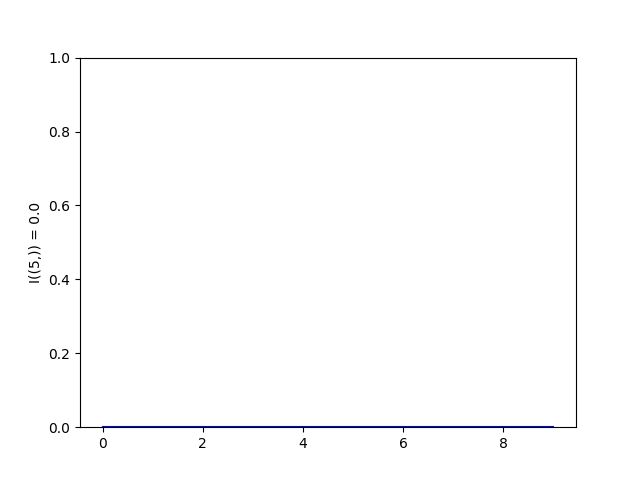
\includegraphics[scale=0.4]{images/1-consistent-partition.png}\hfill
\end{subfigure}
\begin{subfigure}{0.5\linewidth}
\centering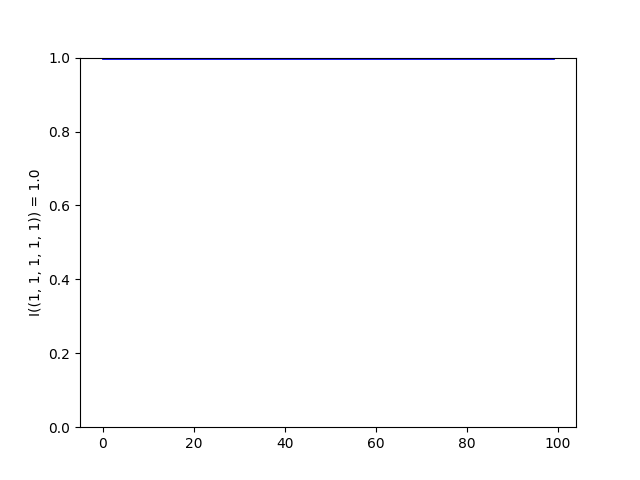
\includegraphics[scale=0.4]{images/1-1-1-1-1-consistent-partitions-probability.png}
\end{subfigure}
\end{figure}

Firstly, it can be seen that for one consistent partition $I(d)$ is equal to $0$ and when the system is fully inconsistent $I(d)$ is equal to $1$.
\begin{figure}

\begin{subfigure}{0.5\linewidth}
\centering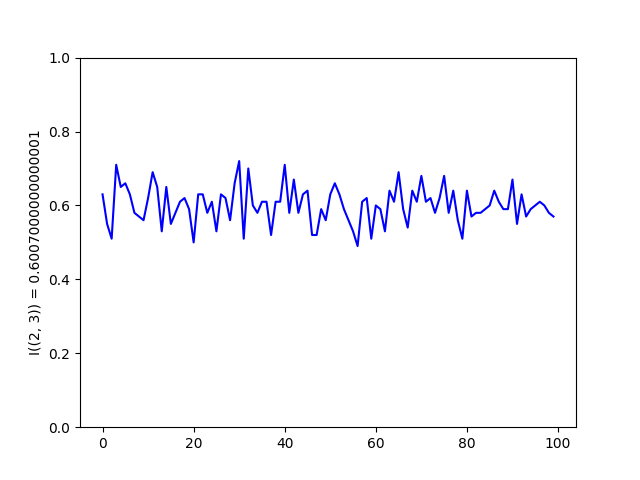
\includegraphics[scale=0.4]{images/2-3-consistent-partitions-probability.png}\hfill
\end{subfigure}
\begin{subfigure}{0.5\linewidth}
\centering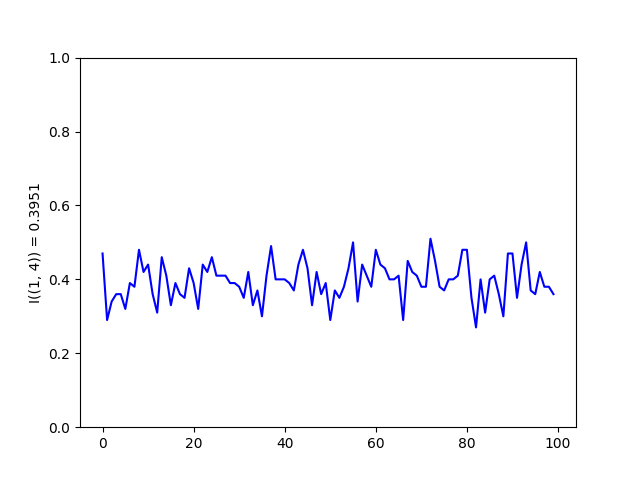
\includegraphics[scale=0.4]{images/1-4-consistent-partitions-probability.png}
\end{subfigure}

Let's compare now the situation when we have two consistent partitions: the set which contains 2 and 3 nodes that consistent in the own subset, and the set with 4 and 1-length consistent subsets.

Then we can easily see that:
\[I(3,2) = 1 - \frac{3 \cdot 2}{5 \cdot 4} - \frac{2 \cdot 1}{5 \cdot 4} = \frac{3}{5} ,\]
and
\[I(4,1) = 1 - \frac{4 \cdot 3}{5 \cdot 4} - \frac{1 \cdot 0}{5 \cdot 4} = \frac{2}{5} ,\]
\end{figure}

Following this procedure for three consistent partitions in $N_d$:

\[I(3,1,1) = 1 - \frac{3 \cdot 2}{5 \cdot 4} - \frac{1 \cdot 0}{5 \cdot 4} - \frac{1 \cdot 0}{5 \cdot 4} = \frac{7}{10} ,\]

and 
\[I(2,2,1) = 1 - \frac{2 \cdot 1}{5 \cdot 4} - \frac{2 \cdot 1}{5  \cdot 4} - \frac{1 \cdot 0}{5 \cdot 4} = \frac{4}{5} .\]


\begin{figure}
\begin{subfigure}{0.5\linewidth}
\centering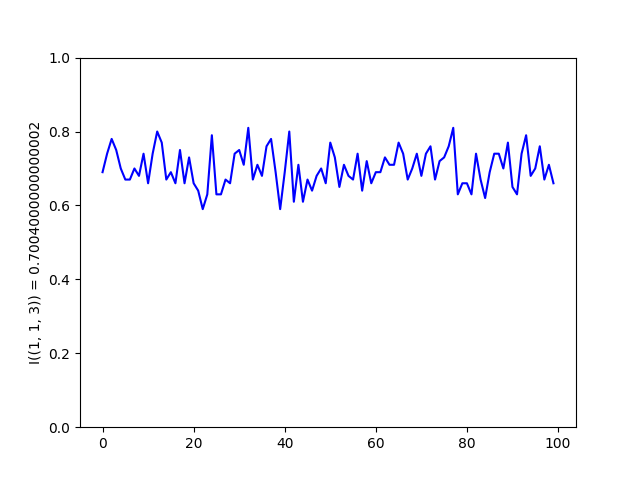
\includegraphics[scale=0.4]{images/1-1-3-consistent-partitions-probability.png}
\end{subfigure}
\begin{subfigure}{0.5\linewidth}
\centering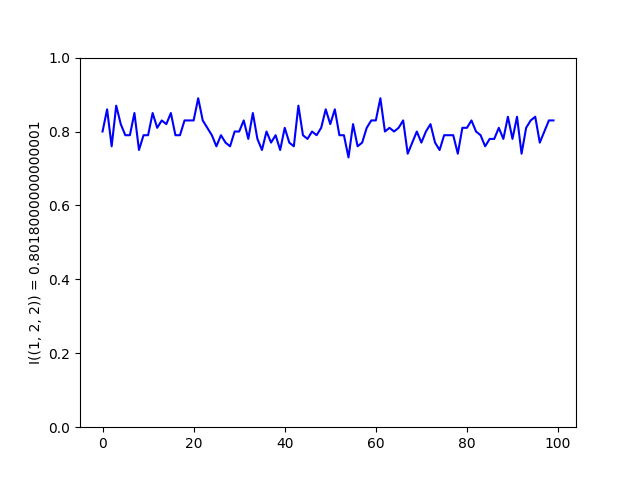
\includegraphics[scale=0.4]{images/1-2-2-consistent-partitions-probability.png}
\end{subfigure}

\end{figure}
And the final one:
\[I(2,1,1,1) = 1 - \frac{2 \cdot 1}{5 \cdot 4} - 3\cdot\frac{1 \cdot 0}{5 \cdot 4} = \frac{9}{10} .\]
\begin{figure}
\begin{subfigure}{0.5\linewidth}
\centering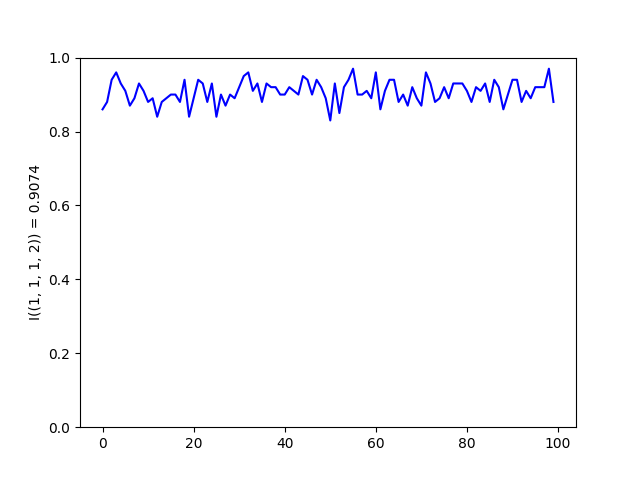
\includegraphics[scale=0.4]{images/1-1-1-2-consistent-partitions-probability.png}
\end{subfigure}
\end{figure}

So, we had easily shown on a simple subset, that our inconsistency metric value corresponds to theoretical one.



Now we present the graphic that demonstrates the verity of that claim we did in previous section about that
consistency convergence time $T_C$ for graph $G$ will be no greater than diameter of $G$.
To be more intuitive, we carried out the set of experiments on our simulation model: having simulated distributed datastore, we easily could run the imitation of one message broadcasting through the datastore and calculate the number of time slots it is taking in the realtime. We have done it for graph with each edge of capacity 1. Below there are graphics for 100, 200, 1000 experiments.
We draw graphics in the following manner: obtain the diameter of graph $G$ (ordinates) and calculated by the simulation $T_c$ (axis). We can easily see that either we have the line demonstrating that $T_C = D(G)$, or
points that are showing that $T_C < D(G)$.

\begin{figure}\label{pic:diagram}
\begin{subfigure}{0.5\linewidth}
\centering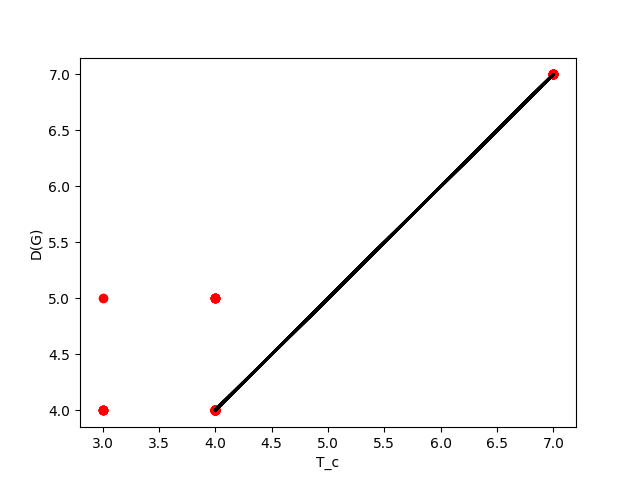
\includegraphics[scale=0.4]{images/100-consistency-convergence.png}
\end{subfigure}
\begin{subfigure}{0.5\linewidth}
\centering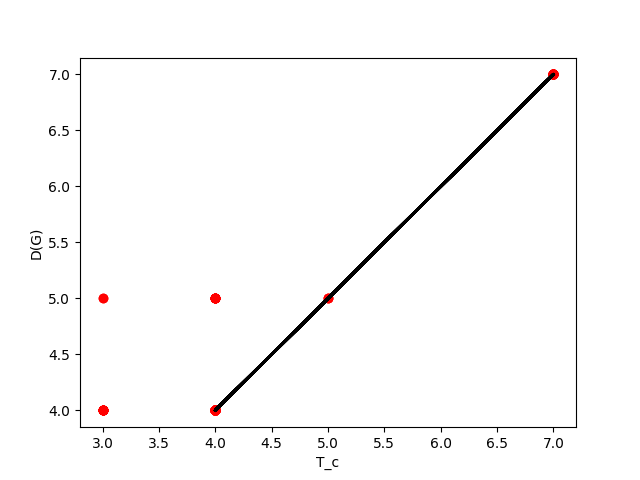
\includegraphics[scale=0.4]{images/200-consistency-convergence.png}
\end{subfigure}
\begin{subfigure}{0.5\linewidth}
\centering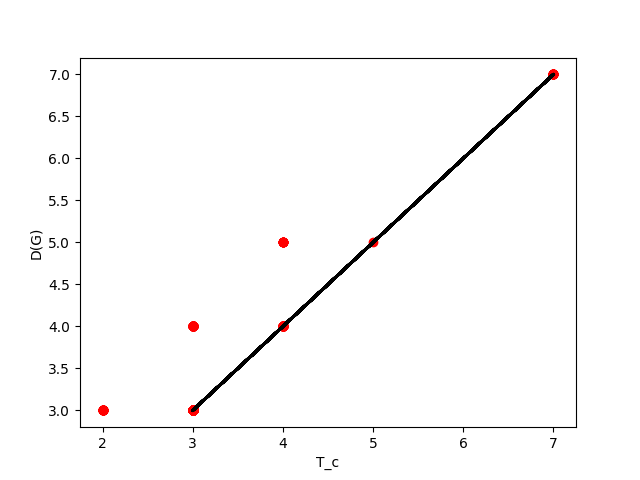
\includegraphics[scale=0.4]{images/1000-consistency-convergence.png}
\end{subfigure}
\end{figure}
\newpage

\section{Simulation Model to Assess Inconsistency Ratio of Data}\label{sec:simulation}

To carry out our experiments, we needed to implement the simulation model that will do experiment and calculate all needed values. This model is implemented as a computer program in Python language. We are thining that it is not valuable to present all the code of the program (however it is available at github page \cite{bib:github_dds}), but we count that it is useful to present the short class diagram of the project.
Look at the picture \ref{pic:diagram} below.

\begin{figure}\label{pic:diagram}
\begin{subfigure}{0.5\linewidth}
\centering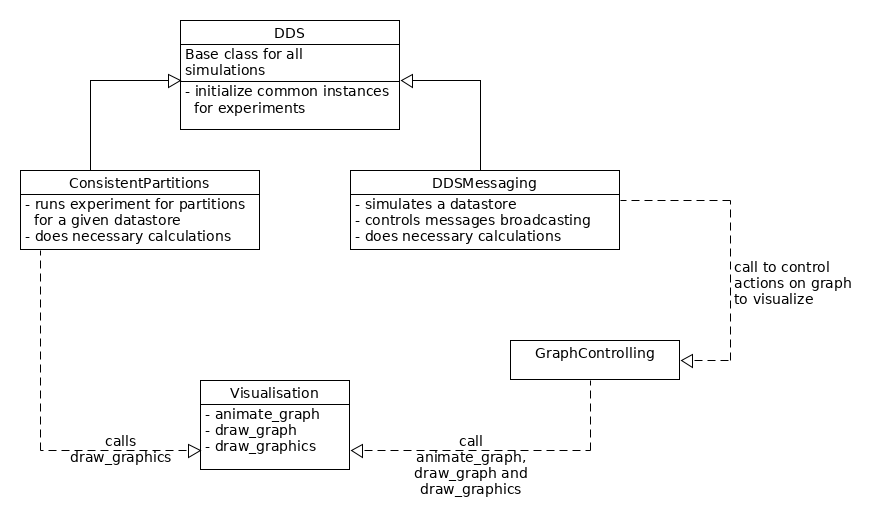
\includegraphics[scale=0.4]{images/dds-class-diagram.png}
\end{subfigure}
\end{figure}


%\section{Replica's actuality research}
%
%We want to calculate the maximum number of compare operations to find inconsistency. Let us imagine that the datastore is fully consistent. This will require comparing all nodes with each other.
%
%Then our sample space looks like:
%
%$\Omega = \{q, qp, qp^2, ..., qp^n\}$
%
%Then the number of comparing operations is:
%
%$\vert\Omega\vert = \sum_{i=0}^{l(N_d)-1}qp^i$
%\\
%
%Obviously, if the storage is consistent, the number of operations will be the maximum. {\color{red}expand - It will allow to calculate the upper, lower boundary, average number of steps could be taken to find if the system is consistent or not.}
%Obviously, if the storage is consistent, the number of operations will be the maximum.
%Then the model will allow to calculate the upper, lower boundary, average number of steps could be
%taken to find if the system is consistent or not.
%
%
%From this formulae we have next constraints:
%\begin{itemize}
%\item The system is fully consistent if $\vert\Omega\vert = l(N_d)-1$
%\item The system is inconsistent when $1 <= \vert\Omega\vert <= l(N_d) -2$
%\end{itemize}
%
%Thus, in the end probability that the node is consistent at time t will be equal to number of consistent nodes (nodes with newest replica versions) $/ l(N_d)$, where $l(N_d)$ is the current length of subset $N_d$ (taking in account that each iteration we put put one node)
%
%Can be combined with number of compare operations.
%Let's also measure the number of steps to find the degree of consistency at a time $t$.
%Our algorithm described above is complemented by that fact that if we find inconsistent nodes,
%we are taking the node with latest replica timestamp. At each node meeting replica version equal to current maximum, we accumulate the count of such nodes. The count is dropped when the new current maximum is found. This is actually the algorithm of search of maximum number in a sequence and has known complexity - $O(N)$ comparisons.
%Then, in our case it is $O(l(N_d))$ steps.



\section{Conclusion}

In this paper we have studied the consistency property for distributed datastores.
So thinking how huge distributed datastores could be and having small interval between write operations to a datastore, we can conclude that binary variable loses its utility.
It might be needed to evaluate current inconsistency state of a datastore, to get nodes that are consistent and make a decision based on obtained results.

Therefore we have proposed stochastic metric instead of binary one considering consistent partitions of a distributed datastore, formed metric for the inconsistency and shown the correctness of the formulae by carrying out experiments, shown when distributed datastore is fully inconsistent and fully consistent, evaluated the upper boundary of time that is taken for consistency convergence in a distributed datastore, taking into account that datastore is reliable, stable and does not have network partitions.


Thus, based on the research of current paper we can make pose following recommendations for those who build the network topology of the distributed datastore:

\begin{itemize}
\item in the case of your datastore is a system with a domination of read operations, it must be sufficient to choose such network topology where frequency of write operations will be no greater than diameter of the graph representing network topology of a distributed datastore;

\item if frequency of write operations is grater than diameter of the graph, it may be useful to evaluate current inconsistency state of the graph;

\item if inconsistency state is close to 0 enough for current requirements, it means that there are inconsistent nodes that are far enough to not conflict with new replicas. Thus, developer or administrator of a datastore  can choose as source availiable for writing that node that is in consistent list and far enough for inconsistent ones. But for that developer needs to provide such an algorithm for a datastore so that he will be able to obtain the current list of consistent nodes;

\item if still more strict consistency needs to be satisfied and inconsitency state is close enough to 0, a developer or administrator of a datastore can choose as source node for writing the node closest to the source node where previous write operation occurred;

\item if replica's history is not important for requirements, it may be possible to solve the problem fixing conflicts. This problem has been investigated in this paper \cite{bib:c_ts}

\end{itemize}


\section{Future work}


In previous section we described that we considered a lot of useful things for consistency in a distributed datastore. But still the research in this direction need to be continued and we have formed the next goals for the the future research:

\begin{itemize}

\item carry out experiments for inconsistency metric in the worst case;

\item complicate a datastore introducing different availability for each node;

\item complicate a datastore introducing various network partitions for a datastore;

\item provide an algorithm that will allow to make a decision what is the best approach for a given datastore such that the eventually consistency is satisfied or an approach when inconsistency will not impact on datastore requirements;

\item theory for finding the most actual replica and time complexity for this algorithm

\item consider all the proposed above metrics in various kinds of real topologies.
\end{itemize}





\begin{thebibliography}{00}


\bibitem{bib:brewer}
Eric A. Brewer:
Towards robust distributed systems,
(Invited talk). Principles of Distributed Computing, Portland, Oregon (July 2000).

\bibitem{bib:prob_approach}
Kyrylo Rukkas, Galyna Zholtkevych:
Distributed Datastores: Towards Probabilistic Approach for Estimation of Dependability,
ICTERI 2015: 523-534

\bibitem{bib:acid_vs_base}
Charles Roe:
ACID vs. BASE: The Shifting pH of Database Transaction Processing
http://www.dataversity.net/acid-vs-base-the-shifting-ph-of-database-transaction-processing, March 1, 2012

\bibitem{bib:tanenbaum}
Tanenbaum, A.S., Van Steen, M.:
Distributed systems. Principles and Paradigms (2nd Edition).
Prentice-Hall, Inc. (2006)

\bibitem{bib:andrews}
Andrews,~G.\,E.:
The theory of partitions.
Addison-Wesley (1976)


\bibitem{bib:github_dds}
G.Zholtkevych: 
DDS Simulation project,
https://github.com/gzholtkevych/DDS-Simulation (2016) 

\bibitem{bib:c_ts}
Sanjay Kumar Madria: 
Handling of Mutual Conflicts in Distributed Databases using Timestamps,
The Computer Journal. Vol. 41, No.\,6 (1998) 

\end{thebibliography}
\end{document}

